\documentclass{beamer} 
\usepackage{tikz}
\usepackage{amsmath,amssymb}
\usepackage{hyperref}
\usepackage{graphicx}

\DeclareMathOperator*{\argmin}{arg\,min}
\DeclareMathOperator*{\Lik}{Lik}
\DeclareMathOperator*{\PoissonLoss}{PoissonLoss}
\DeclareMathOperator*{\Peaks}{Peaks}
\DeclareMathOperator*{\Segments}{Segments}
\DeclareMathOperator*{\argmax}{arg\,max}
\DeclareMathOperator*{\maximize}{maximize}
\DeclareMathOperator*{\minimize}{minimize}
\newcommand{\sign}{\operatorname{sign}}
\newcommand{\RR}{\mathbb R}
\newcommand{\ZZ}{\mathbb Z}
\newcommand{\NN}{\mathbb N}
\newcommand{\z}{$z = 2, 4, 3, 5, 1$} 

\newcommand{\algo}[1]{\textcolor{#1}{#1}}
\definecolor{PDPA}{HTML}{66C2A5}
\definecolor{CDPA}{HTML}{FC8D62}
\definecolor{GPDPA}{HTML}{4D4D4D}

% Set transparency of non-highlighted sections in the table of
% contents slide.
\setbeamertemplate{section in toc shaded}[default][100]
\AtBeginSection[]
{
  \setbeamercolor{section in toc}{fg=red} 
  \setbeamercolor{section in toc shaded}{fg=black} 
  \begin{frame}
    \tableofcontents[currentsection]
  \end{frame}
}

\begin{document}

\title{A tutorial on interpretable machine learning algorithms for understanding factors related to childhood autism}

\author{
  Toby Dylan Hocking\\
  toby.hocking@nau.edu\\
  toby.hocking@r-project.org\\
}

\maketitle

\begin{frame}
  \frametitle{Motivation and data for predicting childhood autism}
  \begin{itemize}
  \item We have National Survey of Children's Health data (NSCH).
  \item Each year a number of people fill out the survey (rows), and
    we have data for their responses (columns).
%download-nsch-data/nsch_2018_topical.do:292:label var k2q35a  "Autism ASD"
  \item One column, k2q35a ``Autism ASD'' (Yes or No) represents if
    the child has Autism.
  \item \textbf{Data pre-processing}: operations prior to machine
    learning.
  \item \textbf{Prediction accuracy in a given year}: can we predict
    Autism variable (output/label/dependent), given the others?
    (inputs/features/independent)
  \item \textbf{Model interpretation / feature selection}: which
    inputs are most useful for prediction?
  \item \textbf{Similarity/difference between years}: Can we train
    on one survey year, and accurately predict on another?
  \end{itemize}
\end{frame}

\begin{frame}
  \frametitle{Machine learning overview and citation}
  \begin{itemize}
  \item In supervised machine learning, train data are paired inputs
    $x$ (images below; survey questions for NSCH) and outputs $y$
    (integer class); goal is accurate prediction on test data.
  \item Hocking TD. Chapter \emph{Introduction to machine learning and neural
    networks} for book \emph{Land Carbon Cycle Modeling: Matrix Approach,
    Data Assimilation, and Ecological Forecasting} edited by Luo Y,
    published by Taylor and Francis (2022).
  \end{itemize}

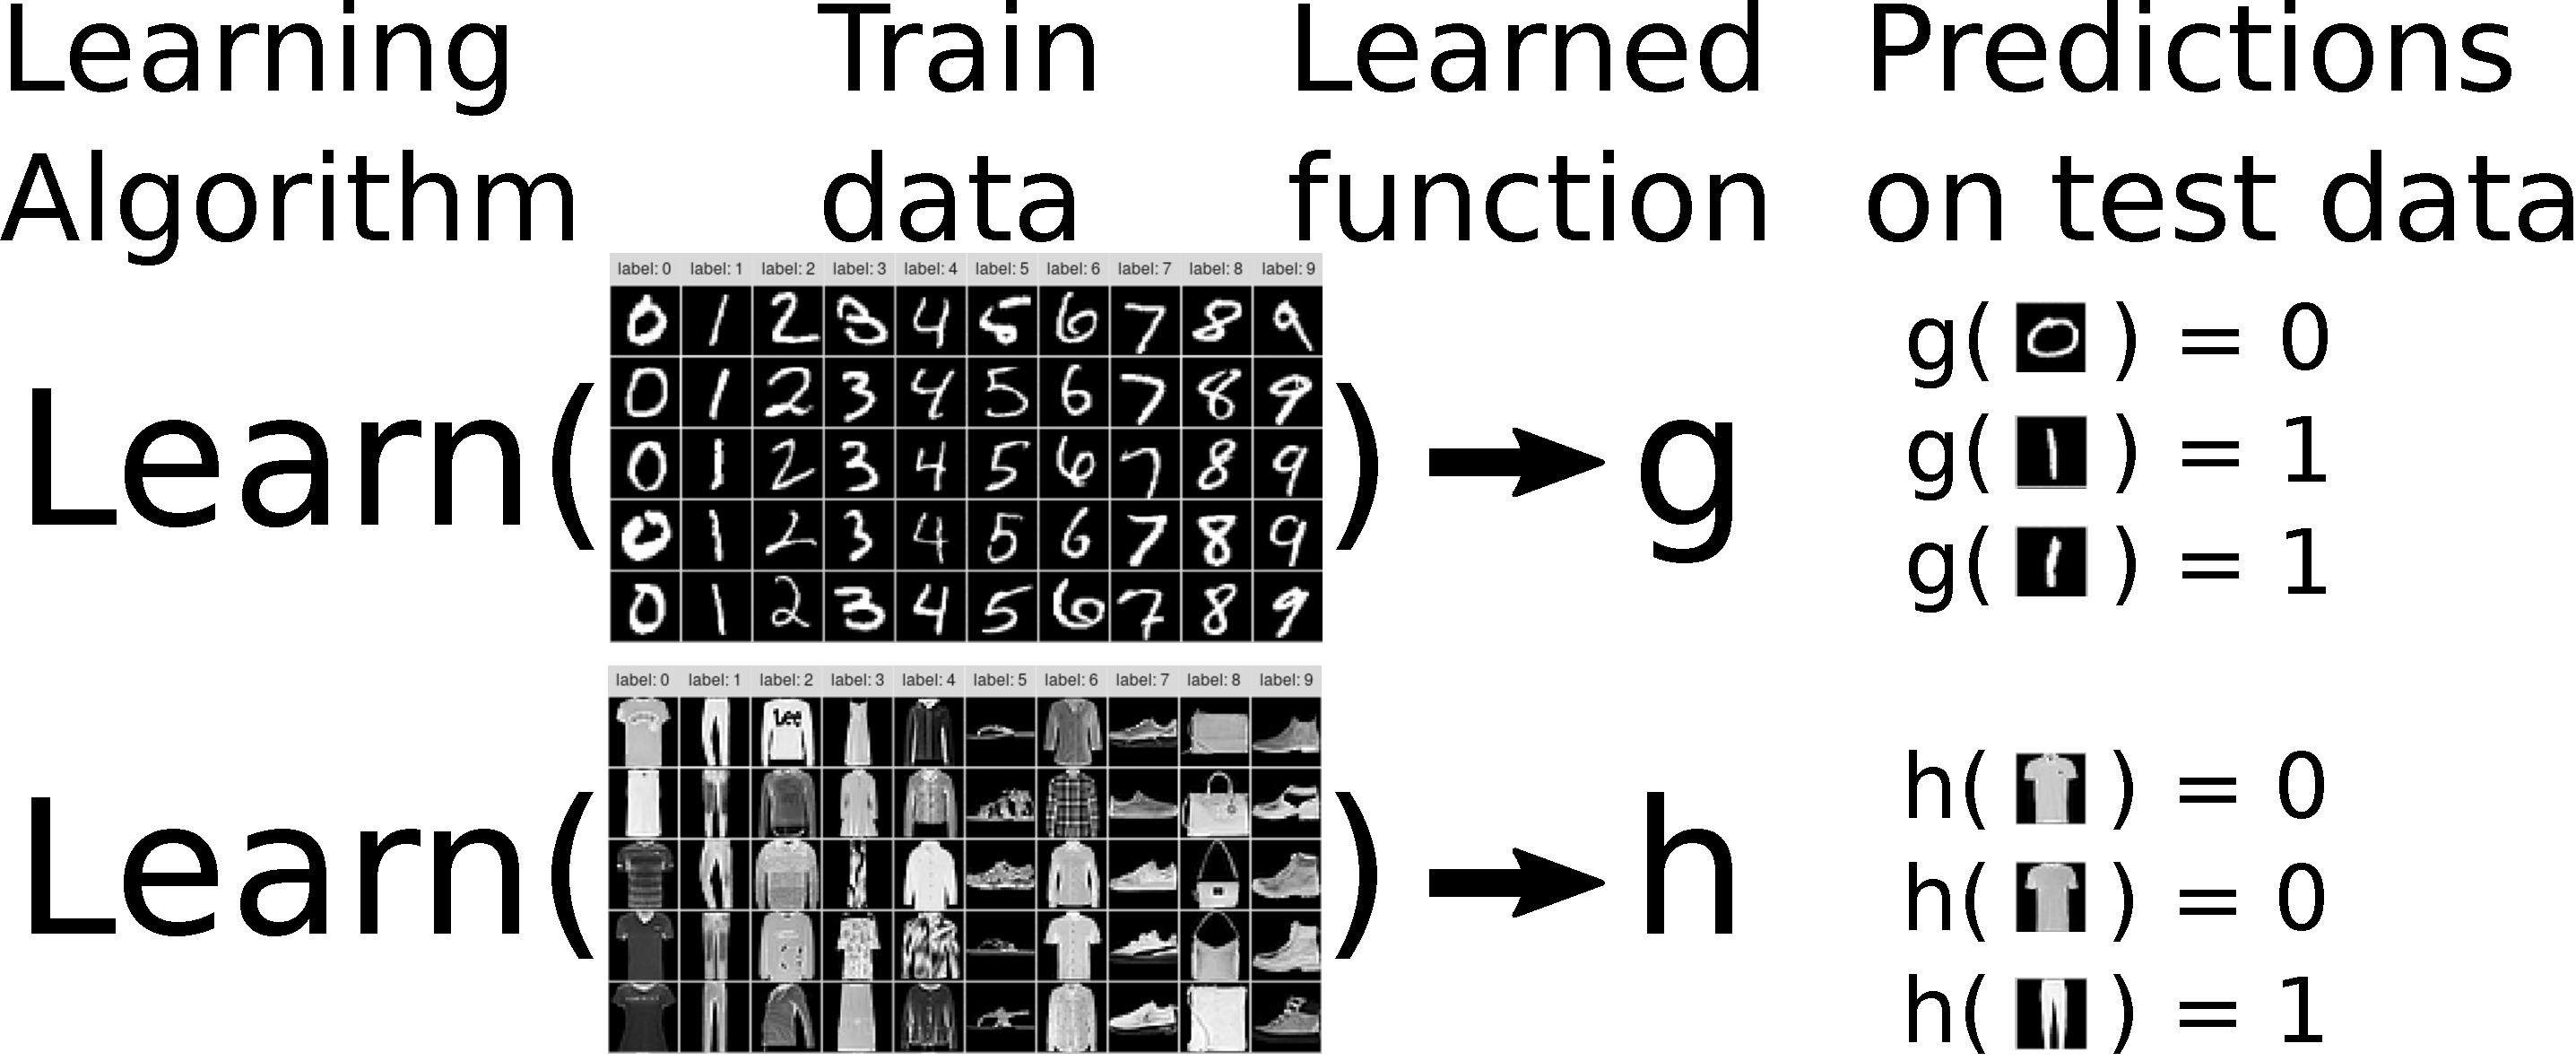
\includegraphics[width=\textwidth]{drawing-mnist-train-test}
\end{frame} 

\section{Data pre-processing}

\begin{frame}
  \frametitle{Data pre-processing overview}

  \begin{itemize}
  \item Goal: for machine learning, need a CSV table with
    rows for people, columns for survey questions.
  \item Download NSCH data from public Census web site.
  \item For each year, keep all columns with less than
    10\% missing values, then remove all rows with at least one missing value.
  \item One-hot recoding of categorical variables (create 0/1
    dummy/indicator variable for each value).
  \item Then keep only columns in common between both years: result is
    46,010 rows and 366 columns. Details:
  \end{itemize}

  \scriptsize
  
  % latex table generated in R 4.3.2 by xtable 1.8-4 package
% Sun Feb 25 15:33:26 2024
\begin{tabular}{rlrrrrrr}
  \hline
year & data.type & nrow & ncol & questions & \%Autism & \%rowsNA & \%colsNA \\ 
  \hline
 2019 & raw & 29433 &   443 &   443 & 2.9615 & 100.0000 & 90.0677 \\ 
   2019 & processed & 18202 &   377 &   187 & 2.9997 & 0.0000 & 0.0000 \\ 
   2020 & raw & 42777 &   443 &   443 & 2.9758 & 100.0000 & 90.0677 \\ 
   2020 & processed & 27808 &   373 &   185 & 3.0818 & 0.0000 & 0.0000 \\ 
   \hline
\end{tabular}
 

Data source:

\url{http://www2.census.gov/programs-surveys/nsch/datasets/2019/nsch_2019_topical_Stata.zip} nsch\_2019\_topical.dta, nsch\_2019\_topical.do

\url{http://www2.census.gov/programs-surveys/nsch/datasets/2020/nsch_2020_topical_Stata.zip} nsch\_2020\_topical.dta, nsch\_2020\_topical.do

\end{frame} 

\begin{frame}[fragile]
  \frametitle{One-hot encoding of categorical variables}

Sometimes called dummy/indicator variables in statistics. 

For each value, we create a new column with 0/1 values.

For example, from \verb|nsch_2020_topical.do|
\begin{verbatim}
label var k4q24_r  "Specialist Visit"
label define k4q24_r_lab  1  "Yes"
label define k4q24_r_lab  2  "No, but this child needed 
 to see a specialist", add
label define k4q24_r_lab  3  "No, this child did not 
 need to see a specialist", add
\end{verbatim}
code above means there is a column named \verb|k4q24_r| in \verb|nsch_2020_topical.dta|, with values 1, 2, 3.

In our analysis we use a one-hot encoding, which means deleting that
column, and creating two 0/1 columns:

\small
\verb|Specialist Visit=Yes| and
\verb|Specialist Visit=No, but this child needed to see a specialist|

\end{frame}

\begin{frame}
  \frametitle{R software citations}
We used the following free/open-source software:
  \begin{description}
  \item[Base R system.] R Core Team (2023). R: A Language and
    Environment for Statistical Computing. R Foundation for
    Statistical Computing, Vienna, Austria.
  \item[Reading Stata dta files in R.]
  Wickham H, Miller E, Smith D (2023). haven: Import and Export
  'SPSS', 'Stata' and 'SAS' Files. R package version 2.5.4.
  \item[Data manipulation, reshaping, summarization.]   
    Barrett T, Dowle M, Srinivasan A, Gorecki J, Chirico M, Hocking T
    (2024). data.table: Extension of data.frame. R package version
    1.15.0.
  \item[Regular expressions for parsing Stata do files in R.] 
    Hocking TD (2023). nc: Named Capture to Data Tables. R package
    version 2023.8.24.
  \item[Data visualization.]
    H. Wickham. ggplot2: Elegant Graphics for Data Analysis.
    Springer-Verlag New York, 2016.
  \end{description}
\end{frame}

\section{Prediction accuracy in a given year}

\begin{frame}
  \frametitle{$K$-fold cross-validation: a standard algorithm used to estimate the prediction accuracy in machine learning}

  \begin{itemize}
  \item $K=3$ folds shown in figure below, meaning three different
    models trained, and three different prediction/test accuracy rates
    computed.
  \item It is important to use several train/test splits, so we can
    see if there are statistically significant differences between
    algorithms.
  \item Rows/observations are people, inputs/features are survey
    questions, and output/label is Autism response (Yes or No).
  \end{itemize}

  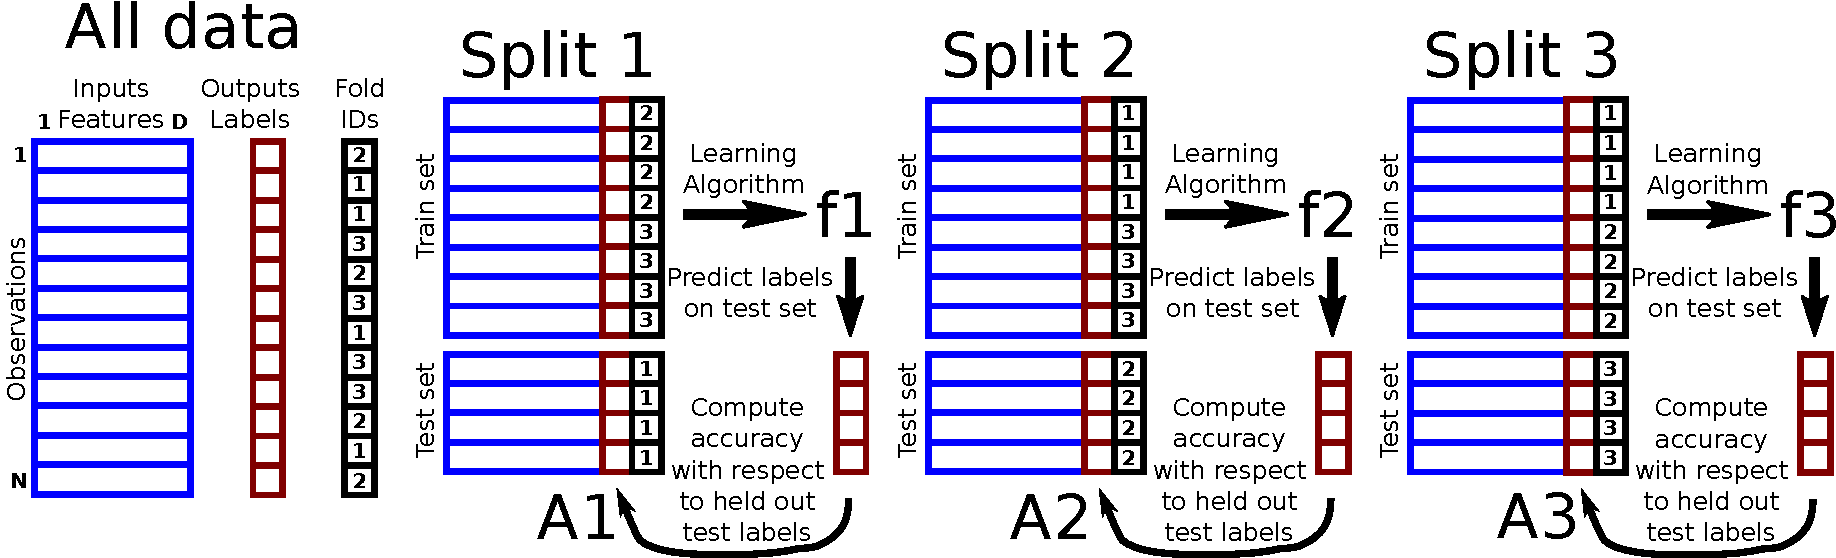
\includegraphics[width=\textwidth]{drawing-cross-validation.pdf}

  \small Hocking TD \emph{Intro. to machine learning and neural
    networks} (2022).
\end{frame}

\begin{frame}
  \frametitle{Learning algorithms we consider}
  We use R packages that implement the following learning
  algorithms, in the mlr3 R package framework:
\begin{description}
\item[cv\_glmnet] L1-regularized linear model (feature
  selection). Friedman, \emph{et al.} (2010).
  % Friedman J, Tibshirani R, Hastie T (2010). “Regularization Paths for
  % Generalized Linear Models via Coordinate Descent.” _Journal of
  % Statistical Software_, *33*(1), 1-22. doi:10.18637/jss.v033.i01
  % <https://doi.org/10.18637/jss.v033.i01>.
\item[xgboost] Extreme gradient boosting (non-linear). Chen and Guestrin (2016). 
\item[rpart] Recursive partitioning, decision tree (non-linear, feature selection). Therneau and Atkinson (2023).
  % Therneau T, Atkinson B (2023). _rpart: Recursive Partitioning and
  % Regression Trees_. R package version 4.1.23,
  % <https://CRAN.R-project.org/package=rpart>.
\item[nearest\_neighbors] classic non-linear algorithm, as implemented
  in kknn R package. Schliep and Hechenbichler (2016).
  % Schliep K, Hechenbichler K (2016). _kknn: Weighted k-Nearest
  % Neighbors_. R package version 1.3.1,
  % <https://CRAN.R-project.org/package=kknn>.
\item[featureless] un-informed baseline, ignores all inputs/features,
  and always predicts the most frequent label in train data (Autism=No
  in our case). Nomenclature from mlr3 R package, Lang, \emph{et al.},
  (2019).
  % Lang M, Binder M, Richter J, Schratz P, Pfisterer F, Coors S, Au Q,
  % Casalicchio G, Kotthoff L, Bischl B (2019). “mlr3: A modern
  % object-oriented machine learning framework in R.” _Journal of Open
  % Source Software_. doi:10.21105/joss.01903
  % <https://doi.org/10.21105/joss.01903>,
  % <https://joss.theoj.org/papers/10.21105/joss.01903>.
\end{description}
Each learning algorithm has different properties (non-linear, feature
selection, etc). For details see Hastie, {\it et al.} (2009) textbook.
\end{frame}

\begin{frame}
  \frametitle{10-fold cross-validation for comparing learning algorithms}
  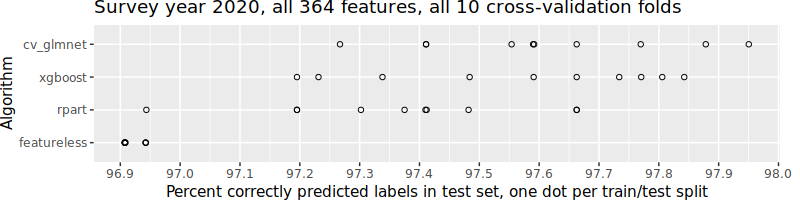
\includegraphics[width=\textwidth]{download-nsch-mlr3batchmark-registry-one-set-all-features.png}

Each dot can be computed in parallel:
\begin{description}
\item[50x speedups] for this figure, 5 algorithms $\times$
  10 cross-validation folds.
\item[NAU Monsoon] super-computer cluster with 4000 CPUs, managed with
  SLURM scheduler software. Typically 50-500x speedups relative to
  sequential computation (1 CPU).
\item[batchtools] R package interface to SLURM system.
\item[mlr3batchmark] R package for running machine learning
  computations in parallel using batchtools.
\end{description}

\end{frame}

\begin{frame}
  \frametitle{Summarize 10 folds with mean and standard deviation}
  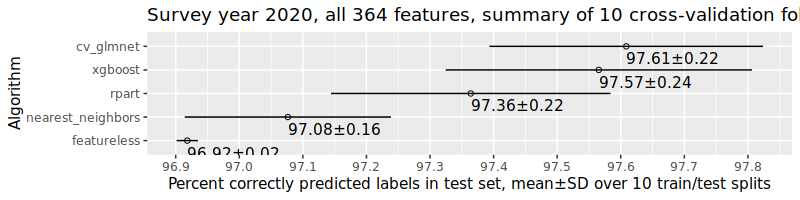
\includegraphics[width=\textwidth]{download-nsch-mlr3batchmark-registry-one-set-all-features-stats.png}

Learning algorithms we consider:
\begin{description}
\item[cv\_glmnet] L1-regularized linear model (feature selection).
\item[xgboost] Extreme gradient boosting (non-linear).
\item[rpart] Recursive partitioning, decision tree (non-linear, feature selection).
\item[nearest\_neighbors] classic non-linear algorithm.
\item[featureless] un-informed baseline, ignores all inputs/features,
  and always predicts the most frequent label in train data (Autism=No
  in our case).
\end{description}

\end{frame}

\begin{frame}
  \frametitle{Confusion matrix and error rates}
  \begin{tabular}{c|c|c}
    & Label 0/No Autism            & Label 1/Yes Autism \\
    \hline
    Predict 0 & True Negative (TN) & False Negative (FN) \\
    \hline
    Predict 1 & False Positive (FP)& True Positive (TP)
  \end{tabular}
  \begin{itemize}
  \item Each has a corresponding rate which is a proportion between
    zero and one, for example FPR=False Positive Rate.
  \item Rates are related, TPR=1-FNR quantifies accuracy for positive
    labels, and TNR=1-FPR is for negative labels.
  \item TN/TP are good (want to maximize), whereas FP/FN are bad (want
    to minimize).
  \item Ideal rates are FPR=0 and TPR=1 but that is not possible to
    achieve in most real data.
  \item Receiver Operating Characteristic (ROC) curves trace TPR as a
    function of FPR, for every threshold of the predicted scores
    $f(x)\in\mathbb R$ (default threshold is typically 0, smaller
    thresholds result in more positive predictions, etc).
  \end{itemize}
\end{frame}

\begin{frame}
  \frametitle{ROC curves show all tradeoffs between TPR and FPR}
  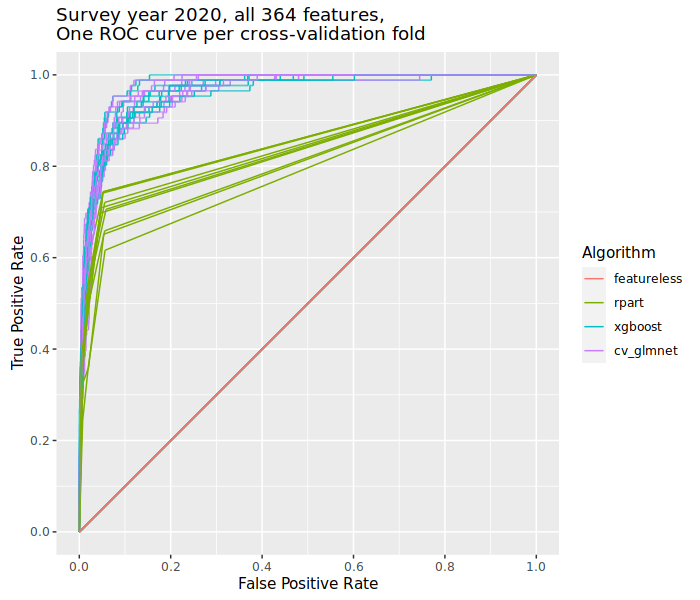
\includegraphics[width=0.9\textwidth]{download-nsch-mlr3batchmark-registry-one-set-all-features-roc.png}
\end{frame}

\begin{frame}
  \frametitle{Default prediction threshold can be viewed as a dot}
  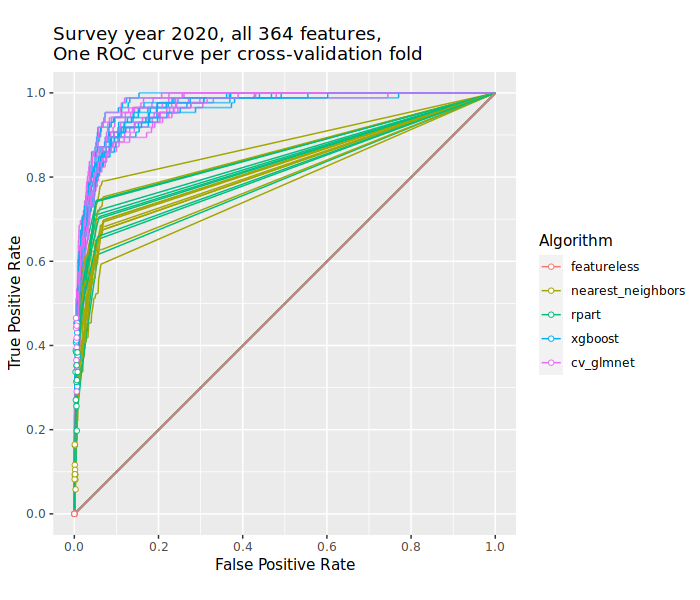
\includegraphics[width=0.9\textwidth]{download-nsch-mlr3batchmark-registry-one-set-all-features-roc-point.png}
\end{frame}

\begin{frame}
  \frametitle{Area Under ROC Curve (AUC) quantifies accuracy over all thresholds}
  \begin{itemize}
  \item Different learning algorithms result in different FPR/TPR at
    default prediction threshold, which can make it difficult to
    fairly compare.
  \item For example, nearest neighbors always had lower FPR/TPR than other
    algorithms.
  \item Is there an algorithm which has a larger TPR, for a given FPR?
    If so, then it is objectively better.
  \item An algorithm with larger AUC means more often larger TPR, for
    a given FPR (averaged over all prediction thresholds).
  \end{itemize}
  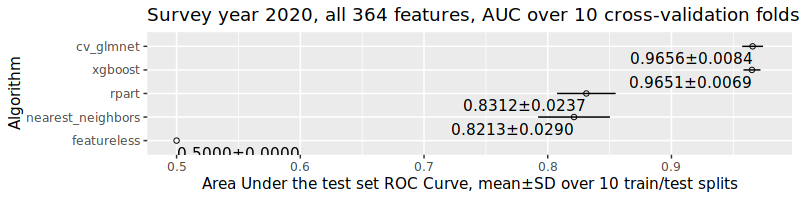
\includegraphics[width=\textwidth]{download-nsch-mlr3batchmark-registry-one-set-all-features-auc.png}
\end{frame}

\section{Model interpretation / feature selection}

\begin{frame}[fragile]
  \frametitle{Column categorization}
Each input/feature column was assigned a category.
\begin{verbatim}
column_name,category
survey_year,
Autism,
State FIPS Code=Alabama,state
...
Number of Children in Household=1,home
...
Sex of Selected Child=Male,birth
...
Deafness=Yes,comorbidity
...
               behavior       birth comorbidity 
          2          15          24          30 
    culture  healthcare        home       state 
         14          88         130          50 
     wealth 
         13 
\end{verbatim}
\end{frame}

\begin{frame}
  \frametitle{Cross-validation for category importance}
  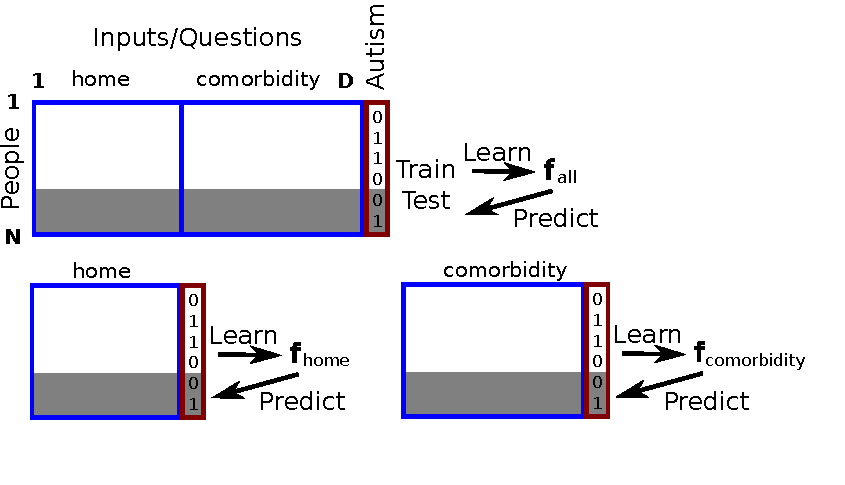
\includegraphics[width=\textwidth]{drawing-cv-feature-sets.pdf}

  \begin{itemize}
  \item Do inputs/questions from home category, or comorbidity
    category, result in more accurate predictions on the test set?
  \end{itemize}
\end{frame}

\begin{frame}
  \frametitle{Cross-validation for category importance}
  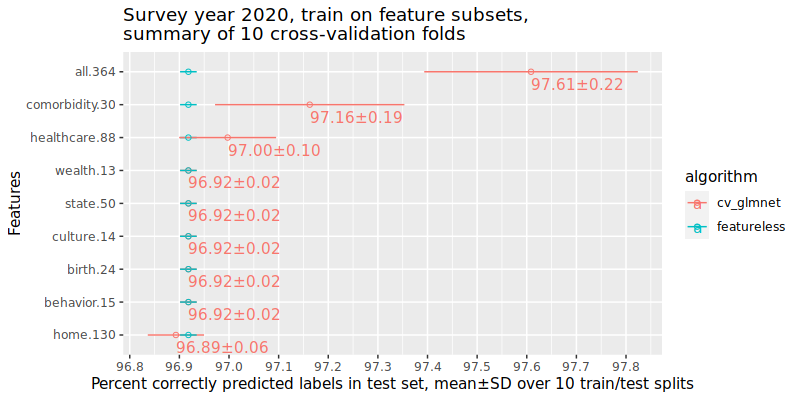
\includegraphics[width=\textwidth]{download-nsch-mlr3batchmark-registry-one-set-compare-features.png}

  \begin{itemize}
  \item None of the categories alone is as accurate as all of the
    features, which implies that some combination of categories is
    required for optimal prediction accuracy.
  \item Co-morbidity is the most accurate single category, and
    healthcare is second; other categories are not useful at all by
    themselves for prediction (same as featureless).
  \end{itemize}

\end{frame}

\begin{frame}
  \frametitle{Linear model coefficient / feature importance}
  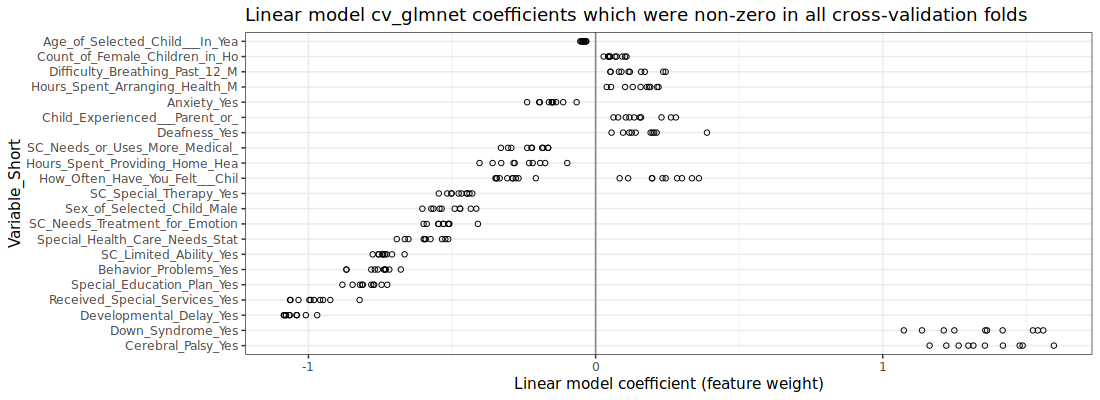
\includegraphics[width=\textwidth]{download-nsch-mlr3batchmark-registry-glmnet-coef-all.png}

  \begin{itemize}
  \item Linear model is
    $\text{Likelihood of autism} = f(x) = \sum_{j=1}^D x_j \beta_j$
    where $x_j$ is input $j$ and $\beta_j$ is the learned weight/coefficient.
  \item For example, above likelihood is 1.4(Cerebral Palsy) + 1.3(Down Syndrome) - 1.1(Developmental Delay)+ ...
  \item Positive weight/coefficient $\beta_j$ means that feature
    contributes to probability of autism=Yes, negative means
    autism=No.
  \item Above we show only most important features, with non-zero
    weights/coefficients in all 10 cross-validation folds (sorted by
    absolute mean weight/coefficient).
  \end{itemize}

\end{frame}

\begin{frame}
  \frametitle{Full figure, variables selected in any number of CV folds}
  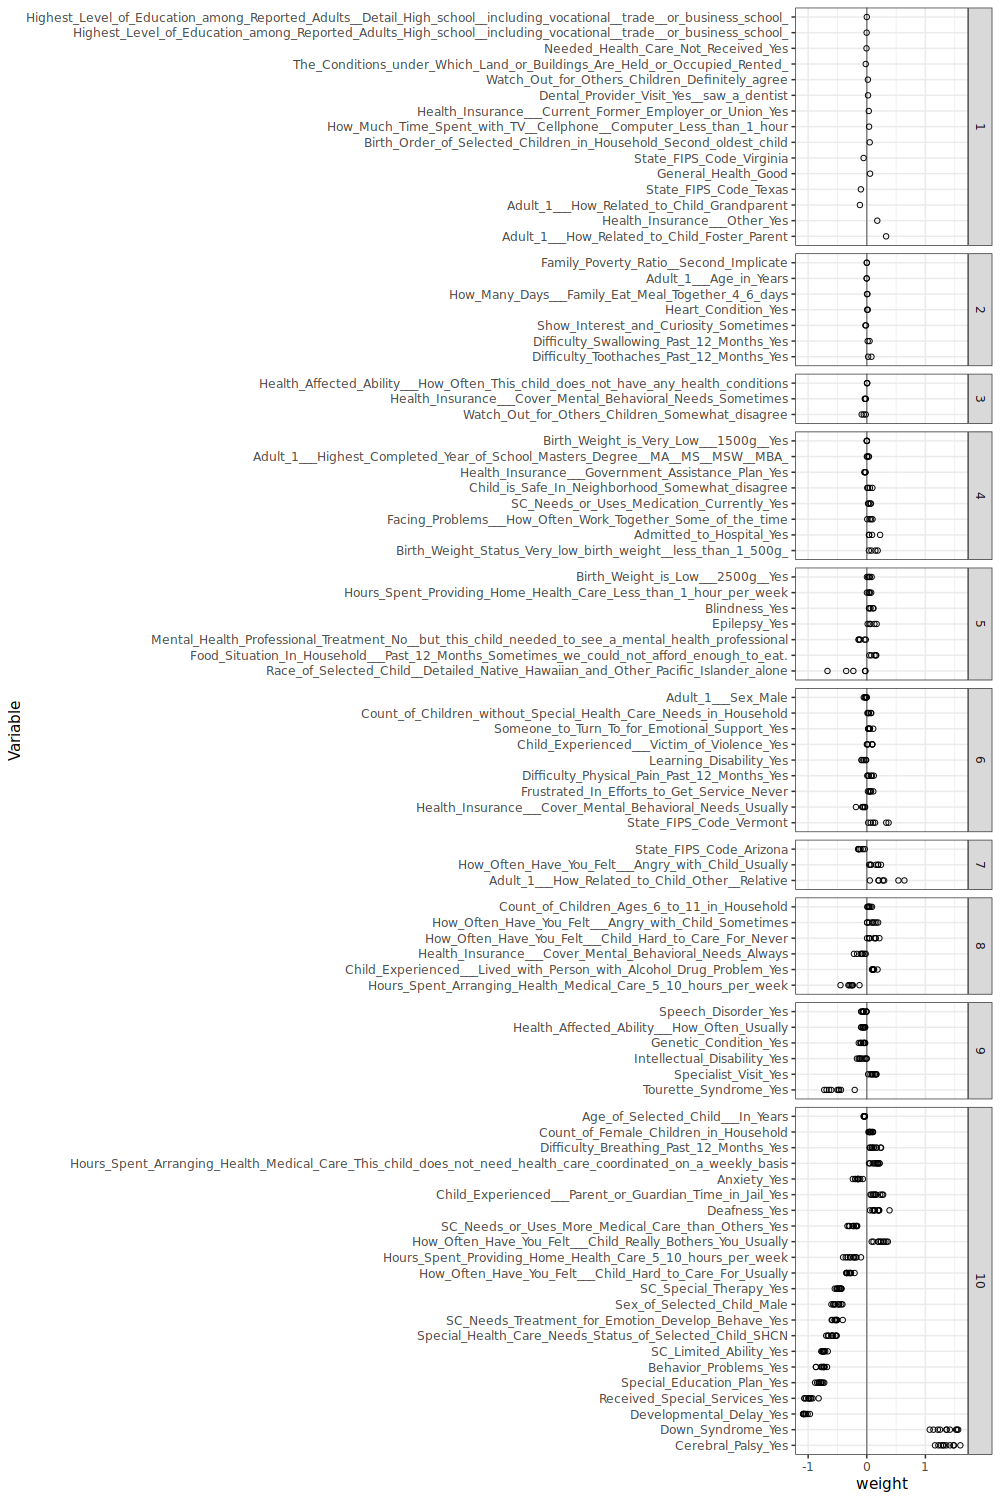
\includegraphics[height=0.7\textheight]{download-nsch-mlr3batchmark-registry-glmnet-coef.png}

  View full figure online, \url{https://github.com/tdhock/2024-01-ml-for-autism/blob/main/download-nsch-mlr3batchmark-registry-glmnet-coef.png}
\end{frame}

\section{Similarity/difference between years}

\begin{frame}
  \frametitle{Cross-validation for determining similarity between years}
  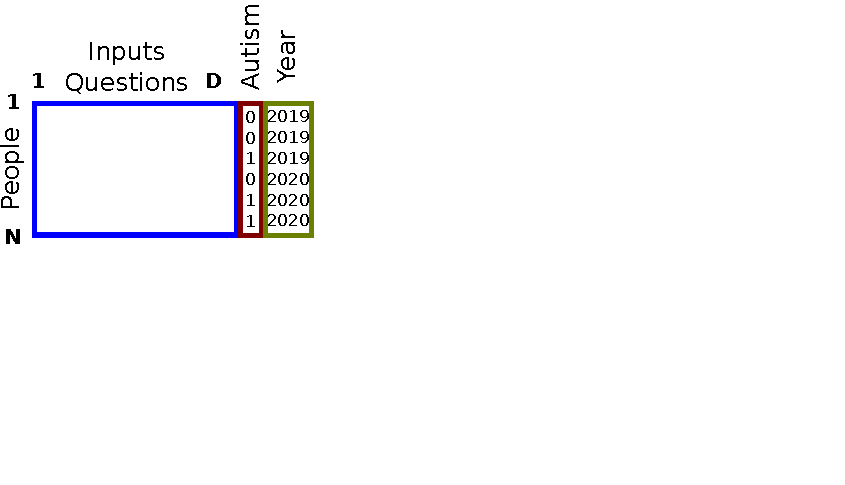
\includegraphics[width=\textwidth]{drawing-cv-same-other-years-1.pdf}
\end{frame}

\begin{frame}
  \frametitle{Cross-validation for determining similarity between years}
  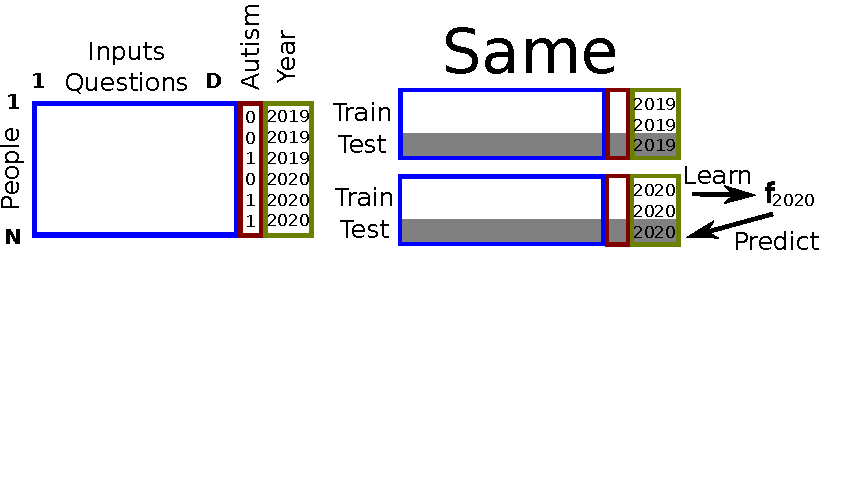
\includegraphics[width=\textwidth]{drawing-cv-same-other-years-2.pdf}
\end{frame}

\begin{frame}
  \frametitle{Cross-validation for determining similarity between years}
  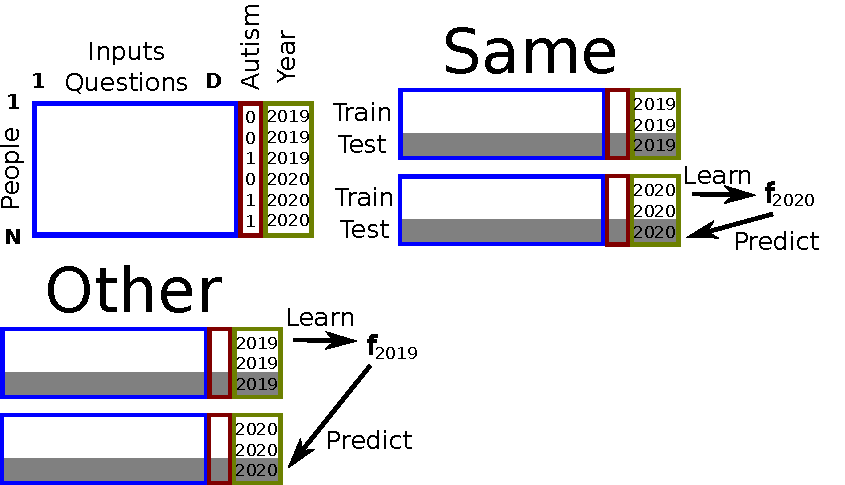
\includegraphics[width=\textwidth]{drawing-cv-same-other-years-3.pdf}
\end{frame}

\begin{frame}
  \frametitle{Cross-validation for determining similarity between years}
  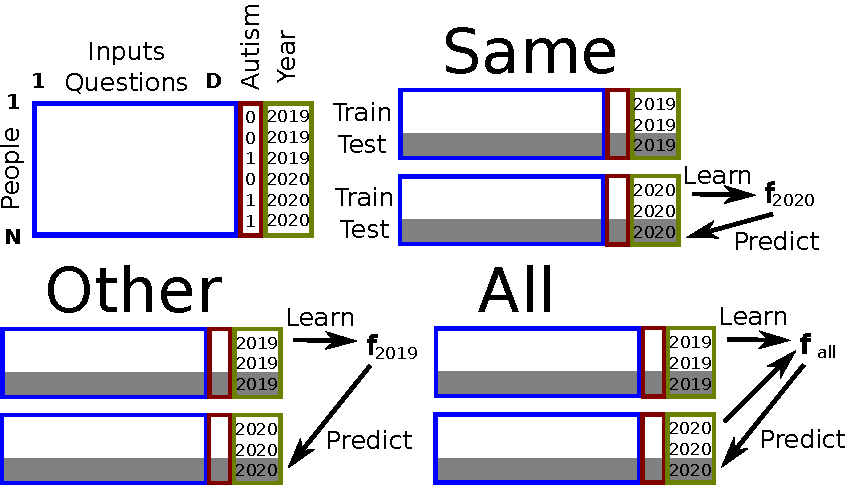
\includegraphics[width=\textwidth]{drawing-cv-same-other-years-4.pdf}
\end{frame}

\begin{frame}
  \frametitle{Cross-validation for determining similarity between years}
  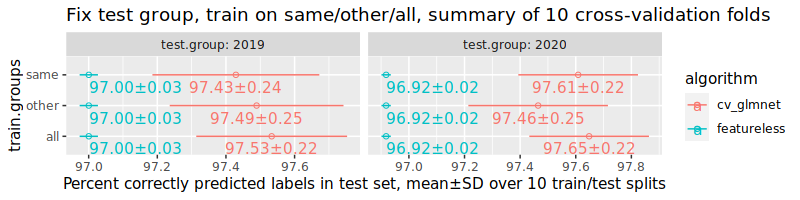
\includegraphics[width=\textwidth]{download-nsch-mlr3batchmark-registry-predict-new-year.png}
  \begin{itemize}
  \item 18,202 rows in 2019, whereas 27,808 in 2020.
  \item For predicting in 2019 (left), training on only 2019 (same) is
    slightly less accurate than training on only 2020 (other), and
    2019+2020 (all). This suggests 2020 data are consistent with the
    pattern in 2019, which is too complex to learn from the limited
    2019 data alone (there is a slight advantage to combining years
    when training).
  \item For predicting in 2020 (right), training on 2019 (other) is slightly less accurate than training on 2020 (same), and 2019+2020 (all). This again suggests that 2019/2020 data are consistent, but there are not enough data in 2019 alone.
  \end{itemize}
% > out.dt[, table(survey_year)]
% survey_year
%  2019  2020 
% 18202 27808 
\end{frame}

\section{Discussion and Conclusions}

\begin{frame}
  \frametitle{Discussion and Conclusions}
  \begin{itemize}
  \item Cross-validation can be used to determine which learning
    algorithms, and features, are most accurate.
  \item Machine learning algorithms like L1 regularized linear models
    (LASSO/cv\_glmnet) are additionally interpretable in terms of
    which features are used for prediction.
  \item Free/open-source software available: mlr3resampling R package
    on CRAN and \url{https://github.com/tdhock/mlr3resampling},
    cross-validation for train on one year, predict on another.
\item These slides are reproducible, using the code in \url{https://github.com/tdhock/2024-01-ml-for-autism}
  \item Contact: toby.hocking@nau.edu,
    toby.hocking@r-project.org
  \end{itemize}
\end{frame}

\begin{frame}
  \frametitle{Default prediction threshold can be viewed as a dot}
  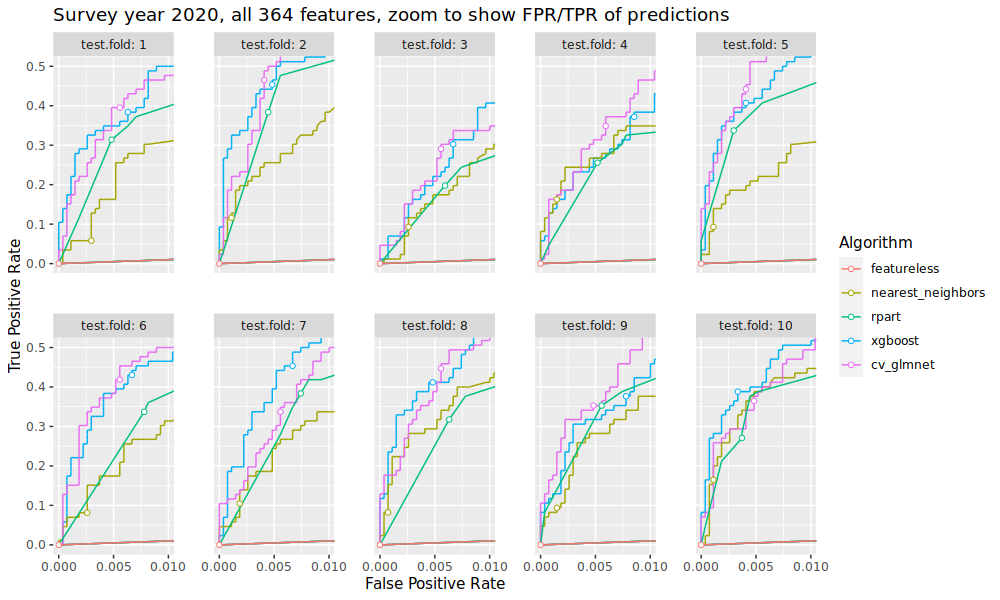
\includegraphics[width=\textwidth]{download-nsch-mlr3batchmark-registry-one-set-all-features-roc-zoom.png}

  Relatively small FPR because there are so few positive labels
  (Autism=Yes only 3\% of 27808 rows in 2020).
% > out.dt[, table(survey_year, Autism)]
%            Autism
% survey_year   Yes    No
%        2019   546 17656
%        2020   857 26951  
% > c2020=c(857, 26951)
% > c2020/sum(c2020)
% [1] 0.03081847 0.96918153
% > sum(c2020)
% [1] 27808
\end{frame}

\begin{frame}
  \frametitle{Cross-validation for determining similarity between years}
  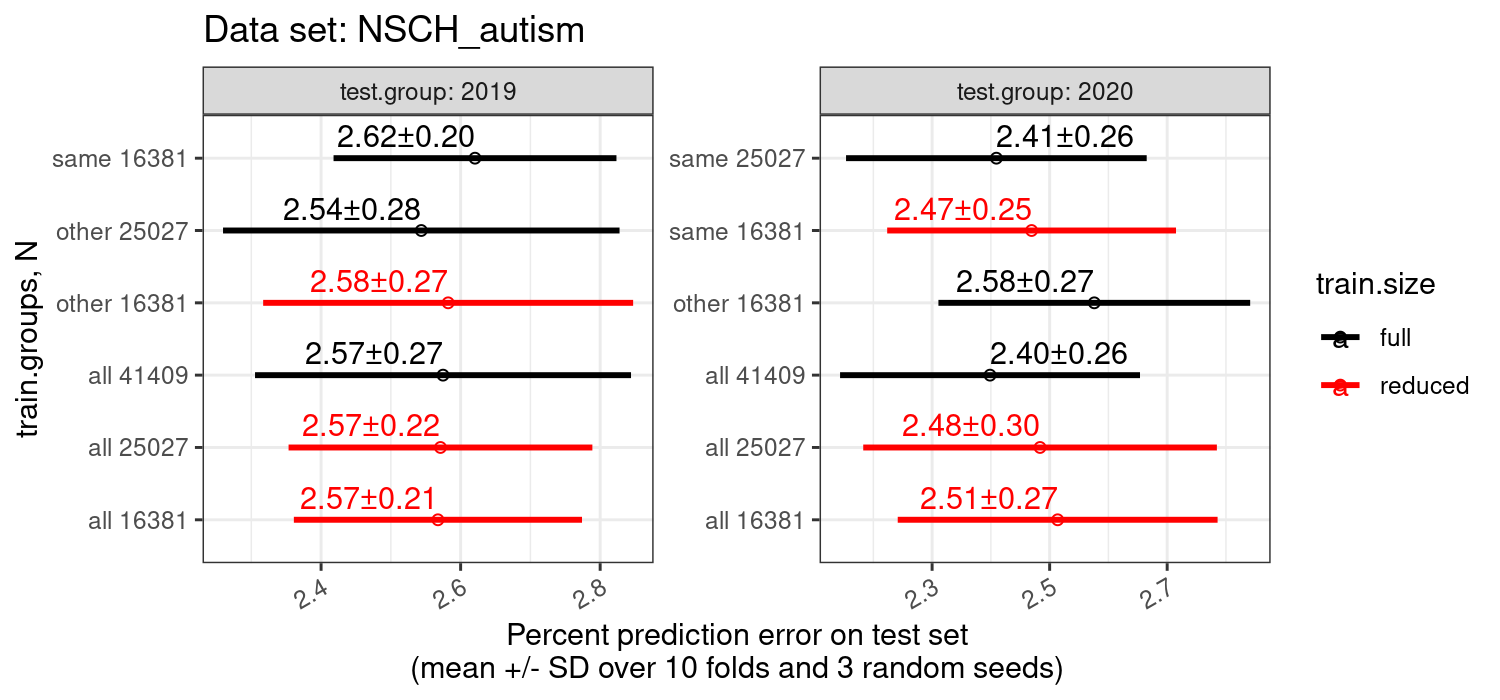
\includegraphics[width=\textwidth]{figures-same-other/NSCH_autism_error_mean_sd_more.png}
  \begin{itemize}
  \item Small dependence on data size in some cases.
  \end{itemize}
\end{frame}

\end{document}

%%% Local Variables:
%%% mode: LaTeX
%%% TeX-master: t
%%% End:
